\documentclass[a4paper,12pt]{article}
\usepackage[T2A]{fontenc}
\usepackage[english]{babel} % языковой пакет
\usepackage{graphicx} % для картинок
\usepackage{amsmath,amsfonts,amssymb} %математика
\usepackage{mathtools}

\usepackage{graphicx}%Вставка картинок правильная
\graphicspath{{Classification.jpg/}{work4-24.jpg/}}

\usepackage{float}%"Плавающие" картинки

\usepackage{wrapfig}%Обтекание фигур (таблиц, картинок и прочего)

\everymath{\displaystyle}

\begin{document}

\section{Лекция 04.10.2024}\label{}
\subsection{Разработка требований}

\subsubsection{Этап...}

\subsubsection{Этап анализа}

\begin{enumerate}
    \item {Классификация}\label{classfic}
    \item Формализация
    \item Анализ качества
\end{enumerate}

Классификация нужна для работы с требованиями; 
целевым форматом оработки (документом); 
формат приема требований



Функциональные требования - то засчет чего будет реализовано действие. 
Все процессы, которые должны быть исполнены в рамках проекта.


Нефункциональные требований - это ограничения о процессах.


Требования детального уровня - могут  


\begin{figure}[h]
    \center{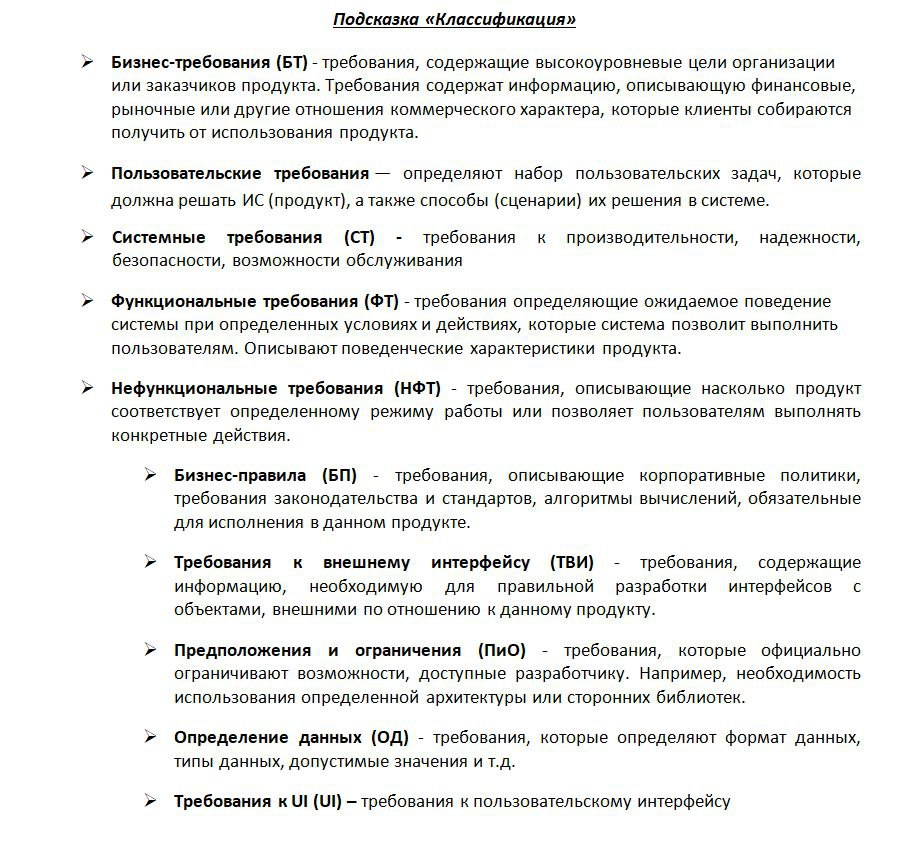
\includegraphics[width=1\linewidth]{Classification.jpg}}
    \caption{Зависимость сигнала от шума для данных.}
    \label{ris:image}
\end{figure}

\begin{figure}[h]
    \center{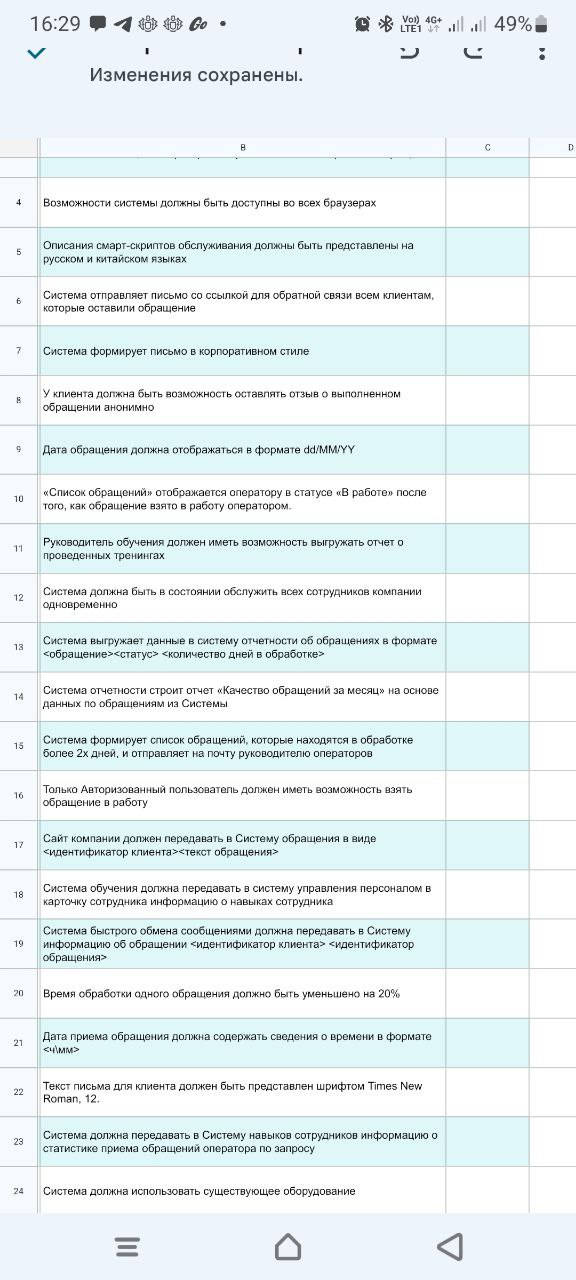
\includegraphics[width=1\linewidth]{work4-24.jpg}}
    \caption{Зависимость сигнала от шума для данных.}
    \label{ris2:image}
\end{figure}


Верхнеуровненые требования - описывают,что нужно, но это не обязательно

7 Детальное, бизнес требование


8 Верхнее требование, пользовательское


9 Детальное, нефункциональное


10 Функциональное требование


11 - Верхний; Пользовательское требование


12 - Системное требование


13 - Детальный уровень, нефункциональные, Определение данных (внешний интерфейс)


14 - Детальный, Функциональное требование


15 - Функциональное


16 - Детальное, нефункциональное, бизнес Требования


17 - Требования к Внешнему интерфейсу


18 - Детальное, можно и Функциональное и не Функциональное


19 - ТВИ


20 - Верхний уровень, Бизнес Требования


21 - детальное, ОД/UI, Нефункциональные


22 - Бизнес правило


23 - Функциональное требование (Тригер процесса)


24 - Системное требование
\subsubsection{Требования и как их Классифицировать}

Все требования можно превратить в функциональные. 
Цели расписываются с помощью верхний и нижних требований.

\subsection{Формализация}

Надо начинать все требования с:


\begin{enumerate}
    \item Необходимо, следует,..>
    \item повысить/понизить/сохранить
    \item точный бизнес-показатель
    \item измеримая величина AS IS - TО BЕ
\end{enumerate}


Заканчивать:


\begin{enumerate}
    \item <Дата, срок, …>
    \item <за счет>
\end{enumerate}


BPMN - 

\subsection{Формализация НФТ/ПТ/СТ}

\begin{enumerate}
    \item возможно отсутствие действия
    \item перечисление свойств/критериев
    \item если действие есть: действительный залог и настоящее время
    \item измеримые данные
    \item дискретность
    \item точность
\end{enumerate}

\subsection{Анализ качества требований}

\begin{enumerate}
    \item Атомарность: Нельзя разделить на несколько требований
    \item Применимость: можно ли связать с другими
    \item Осуществимость: в рамках запланированных бюджета и сроков
    \item Проверяемость: тесткейс из каждого пункта
\end{enumerate}


Скриншот с 4-24 пунктами:


4 - Атомарно, применимо, Не осуществимо, Проверяемость +-


5 - Не атомарно (+-), применимо, осуществимо, Проверяемо


6 - - + + +


7 - 


\end{document}